%%  export TEXINPUTS=.:/home/mjw/src/manuals/common:

\documentclass[11pt,a4paper,openany,oneside]{book}

\usepackage[usenames]{color}
\usepackage{appendix}
\usepackage{dirtree}
\usepackage{epsfig}
\usepackage{fancyhdr}
\usepackage{listings}
\usepackage{graphicx}
\usepackage{parskip}
\usepackage{pifont}
\usepackage{rotating}
\usepackage{enumitem}
\usepackage{latexsym}
\usepackage{titlesec}
\usepackage{xcolor}
\usepackage{fancybox}
\usepackage{caption}
\usepackage{subcaption}
\usepackage{hyperref} % wants to be last

\lstset{
  basicstyle=\ttfamily,
  columns=fullflexible,
  breaklines=true,
  postbreak=\mbox{\textcolor{red}{$\hookrightarrow$}\space},
}

\hypersetup{
  colorlinks   = true, % Colours links instead of ugly boxes
  urlcolor     = blue, % Colour for external hyperlinks
  linkcolor    = blue, % Colour of internal links
  citecolor    = red   % Colour of citations
}

\pagestyle{fancy}
\renewcommand{\chaptermark}[1]{\markboth{\thechapter.\ #1}{}} 
\fancyhead[LE,LO]{\slshape \leftmark}
\fancyhead[RE,RO]{}

% Define some colours
\definecolor{OTTPGreen}{rgb}{0,0.341,0}

% Set formats for each heading level

\titleformat{\chapter}
{}
{\Huge\bfseries\sffamily\color{OTTPGreen}  \thechapter .\space}
{0pt}
{\Huge\bfseries\sffamily\color{OTTPGreen}}

% Change the format of sections
\titleformat*{\section}{\Large\bfseries\sffamily\color{OTTPGreen}}
\titleformat*{\subsection}{\large\bfseries\sffamily\color{OTTPGreen}}
\titleformat*{\subsubsection}{\normalsize\bfseries\sffamily\color{OTTPGreen}}

\newcommand{\ci}[1]{\hspace*{1cm} {\small\texttt{#1}}}
\newcommand{\cc}[1]{{\texttt{#1}}}
\newcommand{\mykey}[1]{{\makebox[16pt] {\put(0,4){\circle{12}} \put(0,4){\makebox(0,0){\small{#1}}}}}}

\newcommand{\sysname}{{TTP}}
\newcommand{\longsysname}{{Time Transfer Platform}}

% Set bullet style
\renewcommand{\labelitemi}{$\Box$} 
\renewcommand{\labelitemii}{$\Box$} 
\renewcommand{\labelitemiii}{$\Box$} 
\renewcommand{\labelitemiv}{$\Box$} 

\newenvironment{description*}%
  {\setlength{\parskip}{0pt}%
	 \begin{description}%
		\setlength{\topsep}{-12pt}%
		\setlength{\itemindent}{-12pt}%
    \setlength{\itemsep}{0pt}%
		\setlength{\itemsep}{0pt}}%
  {\end{description}}

\newenvironment{enumerate*}%
  {\begin{enumerate}%
		\setlength{\topsep}{-12pt}%
		\setlength{\itemindent}{-12pt}%
    \setlength{\itemsep}{0pt}%
		\setlength{\parindent}{0pt}}%
  {\end{enumerate}}
  
\begin{document}

\begin{titlepage}

\begin{center}
\centerline{\includegraphics{figures/ottplogo.png}}
\end{center}

\vspace*{4cm} 

\begin{center}
{\Huge The Open Traceable Time Platform}
\end{center}

\vspace*{4cm} 

\begin{center}
{\Huge User Manual}
\end{center}

\vspace*{4cm}

\begin{center}
Version 2.1.0
\end{center}

\begin{center}
Copyright 2016 E. Louis Marais, Michael Wouters
\end{center}

\begin{center}
Generated \today
\end{center}

\end{titlepage}


\begin{titlepage}

\begin{center}
{\Large This work is licensed under a Creative \\
Commons Attribution 4.0 International License.}
\end{center}

\end{titlepage}

\tableofcontents
\listoffigures
\listoftables

\lstset{
	xleftmargin=24pt,
	basewidth=0.5em,
	basicstyle=\ttfamily,
	escapechar=\%
}

%% ****************************************************************************************
\chapter{Introduction}
%% ****************************************************************************************




This chapter givens a short introduction to the Open Traceable Time Platform (OpenTTP), describing the Reference Platform and other supported hardware.

\section{What is OpenTTP?}

The Open Traceable Time Platform is an open-source solution for a timing system that can be made fully traceable to national standards.
It achieves traceability using the GPS common-view technique, which allows distant clocks to be compared with an accuracy of a few ns.
The reference platform is based on readily available, low-cost OEM modules and provides a full software and hardware solution. 

The goals of the OpenTTP project are:
\begin{enumerate}

	\item Fully open source hardware and software 
	
	\item Easy customisation for specialised applications
	
	\item Production of time-transfer files in the standard CGGTTS data format
	
	\item Easy extension to new receivers

	\item Low cost 

\end{enumerate}

Applications currently include provision of traceable time of day and auditing of NTP-synchronized systems.

\section{The OpenTTP software}

The OpenTTP software provides a full solution for automated logging and processing of time-transfer data.
It is available via GitHub:
\begin{lstlisting}
https://github.com/openttp
\end{lstlisting}
and users are invited to contribute to its development.

The software supports several different GNSS receivers and counter/timers. 
The supported GNSS receivers are mostly low-cost, single-frequency receivers since low cost is a key objective of 
the OpenTTP project.
	
	\subsection{GNSS receivers}
	
	\begin{table}[h]
	\begin{tabular}{lll}
	Manufacturer & models & notes \\ \hline
	Javad & GRIL receivers & obsolete \\
	NVS   & NV08 & \\
	Trimble & Resolution T & obsolete\\
	ublox & Neo8MT & \\
	\end{tabular}
	\caption{Supported GPS/GNSS receivers.}
	\end{table}
	
	Note that OpenTTP uses a custom file format for logging GPS receiver data. It does not read native receiver binary-format files.
	
	Guidance on testing a receiver for suitability for time-transfer, and writing software to process
	the receiver's data, is given in the OpenTTP Developer's Guide.
	
	\subsection{Counter/timers}
	
	\begin{table}[h]
	\begin{tabular}{lll}
	Manufacturer & models & notes \\ \hline
	Agilent & 5313x &  needs IOTech GPIB to RS232 converter\\
	OpenTTP & XEM6001 & \\
	SRS & PRS10 & uses input 1 pps time-tagging function\\
	TAPR & TICC &\\
	\end{tabular}
	\caption{Supported counter/timers.}
	\end{table}
	
\section{The OpenTTP reference platform}

The OpenTTP reference platform consists of:
\begin{itemize}
\item BeagleBone Black, an ARM-based single board computer
\item NVS Technologies NV08-CSM GNSS receiver
\item Opal Kelly XEM6001 FPGA development board
\item Jackson Labs LTE Lite GPS-disciplined oscillator
\item Solid-state disk for mass storage
\item CrystalFontz LCD module
\end{itemize}

Custom circuits, printed circuit board designs and other hardware resources are all available via the GitHub repository.

%% ****************************************************************************************
\chapter{Getting started with the Reference Platform}
%% ****************************************************************************************


This chapter describes basic setup of the OpenTTP reference  platform, verification of its operation and logging in to the unit.

Warning !
The  unit contains a computer. This must be shut down properly
before power is removed from the unit. Failure to do this can 
result in inoperability of the system.
\marginpar{
\epsfig{file=figures/warning.eps,silent=,width=48pt}}
The system can be shut down from the front panel (\ref{sKeypad}) or by
logging in (\ref{sLoggingIn}).


\section{The front panel \label{sFrontPanel}}

\begin{figure}[h]
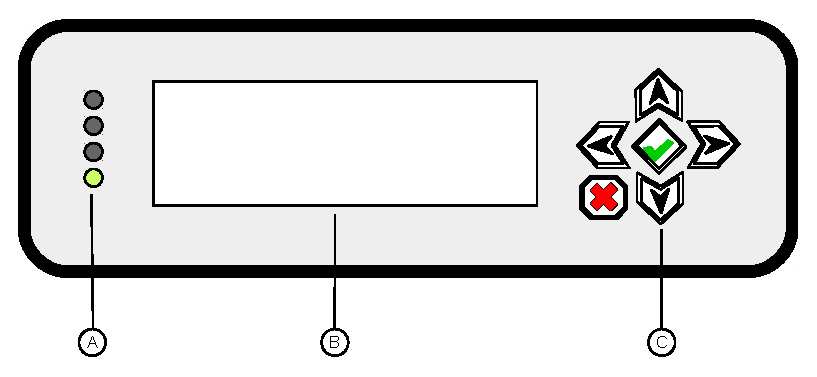
\psfig{file=figures/frontpanel.eps,silent=}
\caption{Front panel of the unit}
\end{figure}

\begin{itemize}
	\item[\mykey{A}] Status LEDs
	\item[\mykey{B}] LCD display
	\item[\mykey{C}] Keypad
\end{itemize}

The top line of the LCD display shows UTC date and time.
The date and time displayed will typically only be accurate to 1 s.
The contents of the second and third lines of the display depend on the display mode
\ref{ss:DisplayMode}.

The bottom line is reserved for notification of system alarms and either shows
`System OK' or `System Alarm'.
The adjacent LED will be red if there is a running alarm.
The other LEDs are currently unused.

\subsection{Using the front panel keypad \label{sKeypad} }

The keypad provides access to status information and limited control and configuration of the unit. 
It can be used to cleanly shut down or reboot the computer without logging in. 

System status is normally displayed on the screen.  
The menus are accessed by pressing any key. Menus are navigated  using the keypad:\\
%%\begin{table}[h]
\begin{tabular}{ll}
 \mykey{\begin{turn}{270}\ding{228}\end{turn}}& Move to next menu item \\
 \mykey{\begin{turn}{90}\ding{228}\end{turn}} & Move to previous menu item \\
 \mykey{\ding{228}}, \mykey{\ding{52}}& Select menu item \\
 \mykey{\begin{turn}{180}\ding{228}\end{turn}}  &Back to previous menu \\
 \mykey{\ding{54}}  & Back to the status display
\end{tabular}
%%\end{table}
\\
Escaping back to the status page after making a change will not undo the change.
Where a sub-menu lists a number of options, the currently selected option is flagged with an asterisk.

Dialogs are navigated using the cursor keys. A dialog will typically consist of a number of input fields.
Some of these work like buttons and are selected using the \mykey{\ding{52}} key; others may require inputting
a value and this is done by cycling through the possible values with the cursor keys.

If you move out of an input field, focus will pass to the next valid input field.

You can quit a dialog using the \mykey{\ding{54}} key. Any changes made in a dialog will not be applied if you quit it.

If a menu or dialog has been inactive for more than 5 minutes, the display returns
to showing system status.

\subsection{Menus}

The menu structure is shown below:

\begin{figure}[ht]
\dirtree{%
 .1 Home screen.
 .2 Setup.
 .3 LCD setup.
 .4 LCD settings.
 .4 LCD backlight time.
 .3 Display mode.
 .4 GPS.
 .4 NTP.
 .4 GPSDO.
 .3 Show IP addresses.
 .2 Show alarms.
 .2 Show system info.
 .2 Restart.
 .3 GPS.
 .3 NTPD.
 .3 Reboot.
 .3 Power down.
}
\caption{Menu structure}
\end{figure}

\subsubsection{LCD setup}

The intensity and contrast of the LCD display can be set using this menu.
A timeout can also be set on the backlight.

\subsubsection{Display mode \label{ss:DisplayMode}}

The status information displayed by the unit in the second and third lines of the LCD display
can be selected as relating to either GPS, NTP or the GPSDO.

When in GPS mode, the identifiers of up
to 10 currently visible GPS space vehicles are displayed. 

When in NTP mode, the second line shows
the number of NTP packets received per minute. The third line shows information about
synchronization status, including leap second announcements.

In GPSDO mode, the second line shows whether the GPSDO is locked or not. 
The third line alternates between the `health' byte (\ref{sGPSDO}), and the estimated fractional frequency error 
(reported by the GPSDO) and the electronic frequency control (EFC) voltage, normalized to a maximum of 100.

\subsubsection{Show alarms}

This shows any currently running alarms as listed in \cc{/home/cvgps/logs/alarms}.

\subsubsection{Show system info}

This displays version and serial number information and the make of the installed oscillator.
This information is read from the file \cc{/usr/local/etc/sysinfo.conf} which has to be manually
updated if the installed oscillator is changed.
  
\subsubsection{Restart}

This allows the user to restart several processes (GPS common view logging and \cc{ntpd}) as well as reboot or power down the unit. 
You will be asked to confirm power down or reboot.

\pagebreak

\section{The rear panel}

%% FIXME need to group these
\begin{figure}[h]
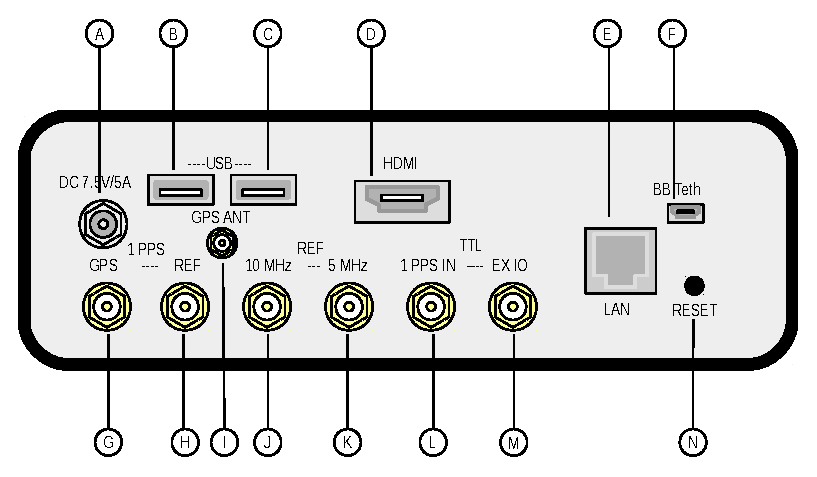
\psfig{file=figures/rearpanel.eps,silent=}
\caption{Rear panel of the unit}
\end{figure}

\begin{table}[h]
	\begin{tabular}{llll}
	& Function & Connector & Signal characteristics \\ 
	\mykey{A} & DC power input & & 7.5 V, 5A \\
	\mykey{B} & USB & & \\
	\mykey{C} & USB & & \\
	\mykey{D} & Video & HDMI & \\
	\mykey{E} & Network & RJ45 & \\
	\mykey{F} & BB USB network & & \\
	\mykey{G} & GPS 1 pps OUT & SMA & 5V DC supplied\\
	\mykey{H} & Reference 1 pps OUT & SMA & \\
	\mykey{I} & GPS antenna & SMB & \\
	\mykey{J} & Reference 10 MHz OUT& SMA & \\
	\mykey{K} & Reference 5 MHz OUT & SMA & \\
	\mykey{L} & 1 PPS IN & SMA & TTL\\
	\mykey{M} & General purpose I/O & SMA & TTL \\
	\mykey{N} & Beaglebone Black reset & &
	\end{tabular}
	\caption{Rear panel electrical connections}
\end{table}

If connected to a computer via the USB connector \mykey{F}, a network adapter should show up on the computer.
The \sysname{} will provide your computer with an IP address of either 192.168.7.1 or 192.168.6.1, depending on the type of USB network adapter
supported by your computer's operating system. The \sysname{} will reserve 192.168.7.2 or 192.168.6.2 for itself.
Further information can be found in the BeagleBone Black documentation.

%% \enlargethispage*{48pt}
%% \pagebreak

\section{Installation}

\subsection{Operating environment}

The \sysname{} is designed for indoor use only and is neither water nor moisture-proof.
It should not be subjected to large mechanical shocks or excessive heat and dust.

\subsection{Install the GPS antenna and cable}

The unit supplies 5 V DC to the antenna. This can be changed to 3.3 V via a jumper J1.
More details are given in \ref{sAntenna}.

The GNSS antenna should be installed in a location with a clear
view of the sky above $10^{\circ}$. All exposed connections should be
weatherproofed. Make sure that all connections are tight but do not apply
excessive torque as this can result in connectors detaching from the cable.

A strain relief bulkhead is  used for making the connection to the short 
`N'-terminated cable. 

\subsection{Make other system connections}


\subsubsection{Network connection}

A network connection is not required for operation as a time-transfer system
but may be useful to the user for maintenance and downloading data files. Otherwise, 
a keyboard and monitor can be plugged in.

For operation as an NTP server, the unit will require a network connection.
The unit can operate using DHCP or with
a static IP address. The default is to use DHCP. The configured address can be conveniently found using the 
front panel menu.

A static IP can be set by using the utility \cc{connmanctl} or by editing the file 
\cc{/etc/network/interfaces}.

\subsubsection{Keyboard and monitor}

A HDMI monitor and USB keyboard and mouse can be used with the \sysname{}. 
However, this only allows a console login \ref{sLoggingIn}.
The graphical login and desktop environment normally available have been disabled to reduce memory usage.


\subsubsection{Time and frequency signals}

Specifications of the various output signals are given in \ref{s:electricalspecs}.

\section{Logging in \label{sLoggingIn}}

The \sysname{} runs under Debian Linux. The desktop environment normally available has been disabled to reduce memory usage.
Familiarity with a command-line Linux environment is therefore essential for operating and maintaining
the \sysname{}. It is beyond the scope of this manual to provide a Linux tutorial. The reader should 
consult one of the many online resources that exist.

Login is via the user \cc{cvgps} (this name is used for historical reasons). 
The default password is supplied separately and you should change
this after logging in.

\section{The cvgps user}

The \cc{cvgps} user is the account used to log and process data.

It contains the following standard directories, some of which are mounted on the SSD.

\begin{figure}[ht]
\dirtree{%
	.1 /home/cvgps.
	.2 bin\DTcomment{executables}.
	.2 etc\DTcomment{configuration files}.
	.2 cggtts.
	.2 logs.
	.3 alarms.
	.2 raw\DTcomment{data files from the receiver, counter, and GPSDO}.
	.2 rinex.
	.2 tmp.
}
\caption{Directories in the \cc{cvgps} account}
\end{figure}

Automatic operation is managed through the \cc{cvgps} \cc{crontab} file \ref{ss:crontab}.
\section{Checking  operation}

Upon startup, a number of alarms may be produced. 
All alarms should clear within five minutes of startup.
Information on alarms and troubleshooting hints are given in \ref{sAlarms}. Troubleshooting
will require logging into the system (\ref{sLoggingIn}).

You can check that logging of GNSS and counter data is occurring by looking in the directory 
\cc{/home/cvgps/raw}.

Processing of data takes place at UTC0015 daily. CGGTTS files will be placed in the 
\cc{/home/cvgps/cggtts} directory.

The \sysname{} is NTP-synchronized using the GPS receiver's time of day messages and its 1 pps. 
The \sysname{} operates on UTC. 
NTP operation can be checked using the command \cc{ntpq -p}. This should display 

\begin{table}
\begin{tabular}{clrrrrrrrr}
     remote      &     refid   &   st & t &  when &poll & reach  &  delay &  offset & jitter \\
% ==============================================================================

\end{tabular}
\caption{Checking NTP operation}
\end{table}

\section{Local configuration}

To produce CGGTTS files, the processing software needs accurate antenna coordinates.
These can be obtained from the \sysname{} receiver, using \cc{navigator}.

\section{Securing the system}

\section{Maintenance}

\subsection{Updating the software}

Debian Linux is updated separately from the OpenTTP software.

Updating the kernel is a separate procedure. 

Updating the OpenTTP software is most conveniently done via the git repository.

\subsection{Replacing the SD card}

To replace the SD card, remove the screws from the front, remove the front panel and disconnect the cable connected to the LCD unit.
Remove the screws at the rear and slide the electronics assembly out. You can remove the SD card without fully removing the electronics.
Insert the new card and reassemble taking care to align the printed circuit boards with the slots in the enclosure.


%% ****************************************************************************************

%% ****************************************************************************************
\chapter{The reference platform hardware}
%% ****************************************************************************************

This chapter provides a more detailed description of the reference platform hardware.


\section{Antenna} \label{sAntenna}

The DC voltage supplied to the antenna is selectable as either 3.3 or 5 V with the jumper J1. 
The default is 5 V. Short circuit protection is 
provided via the $1 \Omega$ fusible resistor R25.

The NV08C-CSM has two antenna inputs ANT-A (active) and ANT-P (passive).
When the antenna is connected to ANT-P (default setting) the external DC power supply is used.
If the antenna is connected to ANT-A, the NV08-CSM board supplies 3.3 V DC and
short circuit protection is provided by the board.


\begin{figure}

	\centering
	
	\begin{subfigure}[t]{6cm}
		\includegraphics[width=6cm]{figures/antennavselpcb.png}
		\caption{Location of JP1 }
	\end{subfigure}
	
	\quad

	\begin{subfigure}[t]{6cm}
		\includegraphics[width=6cm]{figures/antennavselcircuit.png}
		\caption{JP1 voltages}
	\end{subfigure}
	
	\caption{Selection of antenna voltage using JP1}
	
\end{figure}


\begin{figure}
\centerline{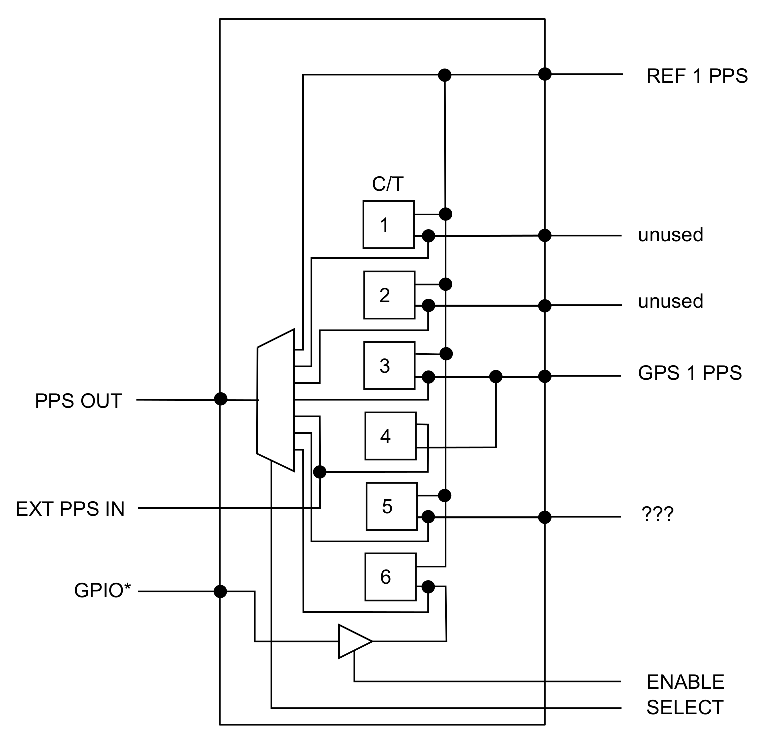
\includegraphics{figures/ottpcounter.eps}}
\end{figure}

\begin{table}
\begin{center}
\begin{tabular}[lll]
1 & channel 1 pps & unused\\
2 & channel 2 pps & GNSS receiver\\
3 & channel 3 pps & unused\\
4 & channel 4 pps & \\
5 & channel 5 pps & \\
6 & channel 6 pps & GPIO\\
7 & GPIO enabled\\
8 & Digital Clock Manager PLL is locked\\
\end{tabular}
\end{center}
\end{table}

\section{Electrical specifications}
\label{s:electricalspecs}

\begin{table}
\begin{tabular}{ll}
GPS 1 pps out & \\
Reference 1 pps out & \\
Reference 10 MHz out & \\
Reference 5 MHz out & \\
1 pps in & \\
General purpose I/O & \\
\end{tabular}
\caption{Electrical signals and their characteristics}
\end{table}

%% ****************************************************************************************
\chapter{Installing the software}
%% ****************************************************************************************
%%
%% \chapter{Software installation}
%% 

\section{Installation requirements}

You will need a basic Linux development environment, including C/C++ compilers, Perl and python2 and python3.
You will likely need the development packages for:
\begin{description*}
	\item[\cc{boost}]  C++ libraries
	\item[\cc{libgsl}] GNU scientific library
\end{description*}

You may also need:
\begin{description*}
	\item[\cc{Time::HiRes}] Perl library
\end{description*}

The above requirements are by no means comprehensive.
What you will need to install will depend very much on the
Linux distribution you are using.

\section{Obtaining, building and installing the software}

The OpenTTP software is obtained from the git repository hosted by GitHub.
There are two main branches, the `master' and `develop' branches.
The `develop' branch is generally stable, but may occasionally be broken.

Clone the repository
\begin{lstlisting}
git clone https://github.com/openttp/openttp.git
\end{lstlisting}
change directory to the repository and then check out the branch you want to use
\begin{lstlisting}
git checkout develop
\end{lstlisting}

\begin{figure}
\dirtree{%
	.1 openttp.
	.2 doc.
	.2 software.
	.3 gpscv.
	.4 common.
	.5 bin.
	.5 etc.
	.5 process.
	.6 mktimetx.
	.5 prs10c.
	.4 gpsdo.
	.4 javad.
	.4 nvs.
	.4 trimble.
	.4 ublox.
	.3 system.
	.4 device-tree-overlays.
	.4 src.
	.5 dioctrl.
	.5 fpga.
	.5 lcdmon.
	.5 libconfigurator.
	.5 ntpd.
	.5 okbitloader.
	.5 okcounterd.
	.5 OpenOK2.
	.5 ppsd.
	.5 sysmonitor.
	.4 udev.
}
\caption{Overview of the OpenTTP software source}
\end{figure}

Two scripts are provided for building and installing the software.
\begin{lstlisting}
software/system/installsys.pl
software/gpscv/install.pl
\end{lstlisting}

The installer has been used with current versions of RedHat Enterprise Linux, 
CentOS, Ubuntu and Debian (on the BeagleBone Black).

\cc{installsys.pl} must be run first (with superuser privileges), 
because it installs libraries which are needed by the GPSCV software.

\cc{installsys.pl} can also be used to install various targets individually.
Run \cc{installsys.pl -h} to see the options available. 
This may be helpful when trying to resolve problems with building the software.

\cc{install.pl} will archive any existing scripts and binaries, and create any
directories it needs in the current user's home directory.

\section{Building the documentation}

The documentation is written in LaTeX and uses some packages and fonts that are generally packaged as `extras'
and will probably need to be installed. The various packages used can be inspected in the file
\cc{doc/manual/OpenTTPManual.tex}.
To build the documentation as a PDF, change directory to \cc{doc/manual} and run \cc{make}.

\section{Common configuration problems}

\subsection{UUCP lock file creation}

UUCP lock files are used to prevent non-OTTP processes from opening serial ports while they are 
in use. You need to set the location for lock file creation specific to the operating system, 
and ensure that the OTTP user (cvgps typically) has the right permissions to write to this location. 
This is typically achieved by adding the user to the appropriate group. 
For example, on Ubuntu 18 the lock directory is \cc{/var/lock}. 
In this case, the directory is world writeable, so 
the OTTP user does not need to belong to any supplementary groups.

\section{A minimal software setup}

For users who wish to use their own hardware,
this section describes the minimum setup required for operation.

The OpenTTP software distribution is comprised of various C/C++ applications and Perl and python scripts.
As a minimum, you will need:
\begin{description*}
	\item \cc{TFLibrary.pm}, a Perl module for commonly used tasks, such as reading configuration files
	\item \cc{ottplib.py}, the \cc{python} version of \cc{TFLibrary.pm}
	\item \cc{libconfigurator}, a C library for parsing configuration files
	\item \cc{lockport}, a utility to create a UUCP lock file
	\item \cc{mktimetx}, to create time-transfer files
	\item one of the OpenTTP-provided scripts to log your receiver
	\item one of the OpenTTP-provided scripts to log your counter/timer
\end{description*}

You must use one of the OpenTTP receiver logging scripts with your GNSS receiver because \cc{mktimetx}
expects a custom file-format \ref{s:DataFileFormat}. In particular, the
receiver's native binary formats are not readable by \cc{mktimetx}. Similarly, OpenTTP uses a custom file
format for the counter-timer measurement files, although in this case, conversion from another format
will probably be straight-forward. Most likely, users will have to provide their own software for
logging their counter/timer, given the large number of possible devices here, and the limited
support within OpenTTP.

You may also find the following useful:
\begin{description*}
	\item[] \cc{kickstart.pl} for automatic start of logging processes
	\item[] \cc{runmktimetx.pl} for automated processing, and reprocessing
	\item[] \cc{gziplogs.pl} for managing log file compression
\end{description*}





%% ****************************************************************************************
\chapter{GPSCV software}
%% ****************************************************************************************


This chapter describes software related to GPSCV time-transfer.

\section{Software overview}


\begin{table}[h]
\begin{tabular}{l|l|l}
	& program & \\ 
	\hline
GPSCV processing  &  & \\
	& \hyperlink{h:mktimetx}{mktimetx} & core program\\
	& \hyperlink{h:runmktimetx}{runmktimetx.pl} & \\
	\hline
TIC logging & & \\
	& \hyperlink{h:hp5313xlog}{hp5313xlog.pl} &\\
	& \hyperlink{h:okxemlog}{okxemlog.pl} & \\
	& \hyperlink{h:prs10log}{prs10log.pl} & \\
	& \hyperlink{h:ticclog}{ticclog.py} & \\
	\hline
GNSS receiver logging & & \\
	&	\hyperlink{h:jnslog}{jnslog.pl} & Javad\\
	& \hyperlink{h:nvslog}{nvslog.pl} & NVS\\
	& \hyperlink{h:restlog}{restlog.pl} & Trimble Resolution T\\
	& \hyperlink{h:ubloxlog}{ubloxlog.pl} & ublox\\
GNSS receiver utilities & & \\
	& \hyperlink{h:restextract}{restextract.pl} & \\
	\hline
Analysis tools & & \\
	& \hyperlink{h:rxdelaycal}{rxdelaycal.pl} & \\
Miscellaneous & & \\
  & \hyperlink{h:log1Wtemp}{log1Wtemp.pl} & \\ 
	\hline
\end{tabular}
\caption{GPSCV software overview}
\end{table}

\section{crontab}

Automatic logging, processing and archival of data is performed through the user \cc{cvgps}' \cc{crontab}.

A minimal \cc{crontab} for the user \cc{cvgps} looks like this:
\begin{lstlisting}
# Check that all logging is running every 5 minutes
*/5 * * * * /usr/local/bin/kickstart.pl # See ~/etc/kickstart.conf

# Run the processing of the data at 00:15
15 0 * * * nice $HOME/bin/runmktimetx.pl >/dev/null 2>&1 

# Give the processing some time to complete, then zip the files at 00:45
45 0 * * * nice $HOME/bin/gziplogs.pl >/dev/null 2>&1

# Check the status of the system once a day, just before the day rollover
56 23 * * * $HOME/bin/checkstatus.pl >$HOME/lockStatusCheck/status.dat
\end{lstlisting}
showing the three essential processes of logging, processing and archival of data.

The active crontab can be examined with the command \cc{crontab -l}. A default \cc{crontab} is
stored in \cc{/home/cvgps/etc/crontab}. 

\section{Configuration file format \label{sConfigFileFormat}}

Configuration files use a common format and are plain text files, designed to be easily edited via a command-line
editor because in many applications, only shell access to the system will be available.

The file is usually divided into sections, with section names delimited by square brackets [ ]. Entries in each section
are of the form:
\begin{lstlisting}
key = value
\end{lstlisting}
For example,
\begin{lstlisting}
[Receiver]
manufacturer = Trimble
model = Resolution T
\end{lstlisting}
defines a section \cc{Receiver} and the two keys: \cc{manufacturer} and \cc{model}. 

The notation \cc{Section::Key} is used to fully specify keys. For example,
\cc{Receiver::model} and \cc{Receiver::manufacturer} specify the two keys above.

Keys and section names are not case-sensitive. Comments begin with a `\#'.

Some keys define a list of sections. For example, the comma-separated list of values for \cc{CGGTTS::outputs} 
\begin{lstlisting}
[CGGTTS]
outputs = C1-code,P1-code,P2-code
\end{lstlisting}
defines three sections: \cc{C1-code}, \cc{P1-code}, and \cc{P2-code}.

\section{Data file formats \label{s:DataFileFormat}}

\subsection{GPS receiver}

This text file records messages from the GPS receiver. The messages can be a mix of ASCII and binary messages.
Binary messages are hexadecimal-encoded. Some logging scripts record ancillary information, 
such as commands sent to the receiver. Comments are allowed, prefaced by a `\#' character. 
The `@' character can be used to tag lines containing special information that needs to be parsed by
the processing software.

Messages are successive lines of the form:
\begin{lstlisting}
<message_id> <time_stamp> <message>
\end{lstlisting}
\textit{Example:}
\begin{lstlisting}
TO 00:00:02 cdfbc75a9a8c353fc5
\end{lstlisting}

Hex encoding of binary messages results in much larger files but these compress to a size not much larger
than the original binary data.

\subsection{Time-interval counter}

This text file records the difference between GNSS receiver and the Reference Oscillator 1 pps,
measured each second. Entries are successive lines of the form:
\begin{lstlisting}
<time_of_day> <time_difference>
\end{lstlisting}
where the time difference is in seconds.\\
\textit{Example:}
\begin{lstlisting}
00:00:04  +4.0821E-006 
\end{lstlisting}


\section{gpscv.conf - the core configuration file \label{sgpscvconf} }

A single configuration file, \cc{gpscv.conf}, provides configuration information to most of the
OpenTTP software. 
\cc{gpscv.conf} is used by \cc{mktimetx}, receiver logging scripts, TIC logging scripts,receiver utilities and so on.

It uses the format described in \ref{sConfigFileFormat}.

\begin{table}[h]
\begin{tabular}{l|p{10cm}}
Section & Key \\ \hline
\hyperlink{h:antenna}{Antenna} & antenna number, antenna type, 
				delta H, delta N, delta E, frame,
				marker name, marker number,
				X, Y, Z\\ \hline
\hyperlink{h:cggtts}{CGGTTS} & BIPM cal id, comments, create, 
         ephemeris, ephemeris file, ephemeris path,
         internal delay, lab id, maximum DSG, minimum elevation,
         minimum track length, naming convention, outputs, reference,
         receiver id, revision date, version,
         code, constellation, path
         \\ \hline
\hyperlink{h:delays}{Delays}  & antenna cable, reference cable 
         \\ \hline
\hyperlink{h:counter}{Counter} & file extension, GPIB address, header generator, lock file,
         logger, logger options, okxem channel, port
				\\ \hline
\hyperlink{h:misc}{Misc}    & gzip
				\\ \hline
\hyperlink{h:paths}{Paths} & CGGTTS, counter data, processing log, receiver data, RINEX, tmp
				\\ \hline
\hyperlink{h:receiver}{Receiver} & configuration, elevation mask, logger, logger options, 
				 manufacturer, model, observations, 
         port, pps offset, synchronization, pps synchronization delay,
         status file, timeout, version
				\\ \hline
\hyperlink{h:reference}{Reference} & file extension, logging interval, log path, log status, oscillator, power flag, status file
        \\ \hline
\hyperlink{h:rinex}{RINEX}  & agency, create, observer, version
				\\ \hline
\end{tabular}
\caption{Summary of \cc{gpscv.conf} entries}
\end{table}

\subsection{[Antenna] section}

\hypertarget{h:antenna}{}
{\bfseries antenna number}\\
This appears as ANTNUM in the RINEX header.\\
\textit{Example:}
\begin{lstlisting}
antenna number=A567456
\end{lstlisting}

{\bfseries antenna type}\\
This appears as ANTTYPE in the RINEX header.\\
\textit{Example:}
\begin{lstlisting}
antenna type=Ashtec
\end{lstlisting}

{\bfseries delta H}\\
This appears as DELTA H in the RINEX header.\\
\textit{Example:}
\begin{lstlisting}
delta H=0.0
\end{lstlisting}

{\bfseries delta E}\\
This appears as DELTA E in the RINEX header.\\
\textit{Example:}
\begin{lstlisting}
delta E=0.0
\end{lstlisting}

{\bfseries delta N}\\
This appears as DELTA N in the RINEX header.\\
\textit{Example:}
\begin{lstlisting}
delta N=0.0
\end{lstlisting}

{\bfseries frame}\\
This appears as FRAME in the CGGTTS header.\\
\textit{Example:}
\begin{lstlisting}
frame= ITRF2010
\end{lstlisting}

{\bfseries marker name}\\
This appears as MARKER NAME in the RINEX header.\\
\textit{Example:}
\begin{lstlisting}
marker name=
\end{lstlisting}

{\bfseries marker number}\\
This appears as MARKER NUMBER in the RINEX header.\\
\textit{Example:}
\begin{lstlisting}
marker number=
\end{lstlisting}

{\bfseries X}\\
This appears as X in the CGGTTS header and APPROX POSITION XYZ in the RINEXheader.\\
\textit{Example:}
\begin{lstlisting}
X=+4567890.123
\end{lstlisting}

{\bfseries Y}\\
This appears as Y in the CGGTTS header and APPROX POSITION XYZ in the RINEXheader.\\
\textit{Example:}
\begin{lstlisting}
Y=+2345678.90
\end{lstlisting}

{\bfseries Z}\\
This appears as Z in the CGGTTS header and APPROX POSITION XYZ in the RINEXheader.\\
\textit{Example:}
\begin{lstlisting}
Z=-1234567.890 
\end{lstlisting}


\subsection{[CGGTTS] section }

\hypertarget{h:cggtts}{Entries} in this section control the format and content of CGGTTS files and filtering applied to CGGTTS tracks.

{\bfseries BIPM cal id}\\
This defines CAL\_ID for the internal delay, as used in v2E CGGTTS headers.\\
\textit{Example:}
\begin{lstlisting}
BIPM cal id=none
\end{lstlisting}

{\bfseries comments}\\
This defines COMMENTS in the CGGTTS header.\\
\textit{Example:}
\begin{lstlisting}
comments=none
\end{lstlisting}

{\bfseries create}\\
This defines whether or not CGGTTS files will be generated.\\
\textit{Example:}
\begin{lstlisting}
create=yes
\end{lstlisting}

{\bfseries ephemeris}\\
This defines whether to use the receiver-provided ephemeris or a user-provided ephemeris (via a RINEX navigation file).
If a user-provided ephemeris is specified then \cc{ephemeris path} and \cc{ephemeris file} 
must also be specified.\\
\textit{Example:}
\begin{lstlisting}
ephemeris=receiver
\end{lstlisting}

{\bfseries ephemeris file}\\
This specifies a pattern for user-provided RINEX navigation files.
Currently, only patterns of the form \cc{XXXXddd0.yyn} are recognized.\\
\textit{Example:}
\begin{lstlisting}
ephemeris file=SYDNddd0.yyn
\end{lstlisting}

{\bfseries ephemeris path}\\
This specifies the path to user-provided RINEX navigation files.\\
\textit{Example:}
\begin{lstlisting}
ephemeris path=igsproducts
\end{lstlisting}

{\bfseries internal delay}\\
This defines INT DLY in the CGGTTS header. The units are ns.\\
\textit{Example:}
\begin{lstlisting}
INT DLY=0.0
\end{lstlisting}

{\bfseries lab id}\\
This defines the two-character lab code used for creating BIPM-style file names, as per the V2E specification.\\
\textit{Example:}
\begin{lstlisting}
lab id=AU
\end{lstlisting}

{\bfseries maximum DSG}\\
CGGTTS tracks with DSG lower than this will be filtered out. 
The units are ns.\\
\textit{Example:}
\begin{lstlisting}
maximum DSG = 10.0
\end{lstlisting}

{\bfseries minimum elevation}\\
CGGTTS tracks lower than this will be filtered out. 
The units are degrees.\\
\textit{Example:}
\begin{lstlisting}
minimum elevation = 10
\end{lstlisting}

{\bfseries minimum track length}\\
CGGTTS tracks shorter than this will be filtered out. Tracks meeting the criterion are not necessarily contiguous.
The units are seconds.\\
\textit{Example:}
\begin{lstlisting}
minimum track length = 390
\end{lstlisting}

{\bfseries naming convention}\\
Defines the CGGTTS file naming convention. Valid options are `plain' (MJD.cctf) and `BIPM'.
The \cc{lab id} and \cc{receiver id} should be defined in conjunction with BIPM-style filenames.\\
\textit{Example:}
\begin{lstlisting}
naming convention = BIPM
\end{lstlisting}

{\bfseries outputs}\\
This defines a list of sections which in turn define the desired CGGTTS outputs.\\
\textit{Example:}
\begin{lstlisting}
outputs=CGGTTS-GPS-C1,CGGTTS-GPS-P1,CGGTTS-GPS-P2
\end{lstlisting}

{\bfseries reference}\\
This defines REF in the CGGTTS header.\\
\textit{Example:}
\begin{lstlisting}
reference=UTC(XXX)
\end{lstlisting}

{\bfseries receiver id}\\
This defines the two-character receiver code used for creating BIPM-style file names, 
as per the V2E specification.\\
\textit{Example:}
\begin{lstlisting}
receiver is=01
\end{lstlisting}

{\bfseries revision date}\\
This defines REV DATE in the CGGTTS header. It must be in the format YYYY-MM-DD.\\
\textit{Example:}
\begin{lstlisting}
revision date = 2015-12-31
\end{lstlisting}

{\bfseries version}\\
This defines the version of CGGTTS output.Valid versions are v1 and v2E. 
The \cc{lab id} and \cc{receiver id} should be defined in conjunction with v2E ouput\\
\textit{Example:}
\begin{lstlisting}
version = v2E
\end{lstlisting}

\subsubsection{CGGTTS output sections}

Multiple CGGTTS outputs can be defined, allowing for different constellation and signal combinations.
An example of a CGGTTS output section is as follows:
\begin{lstlisting}
[CGGTTS-GPS-C1]
constellation=GPS
code=C1
path=cggtts
BIPM cal id = none
internal delay = 11.0
\end{lstlisting}

The new entries for a CGGTTS output section are:\\
{\bfseries code}\\
This defines the GNSS signal code. Valid values are C1,P1 and P2.\\
\textit{Example:}
\begin{lstlisting}
code=C1
\end{lstlisting}

{\bfseries constellation}\\
This defines the GNSS constellation. Only GPS is supported currently.\\
\textit{Example:}
\begin{lstlisting}
constellation=GPS
\end{lstlisting}

{\bfseries path}\\
This defines the directory in which output files are placed.\\
\textit{Example:}
\begin{lstlisting}
path=cggtts
\end{lstlisting}

\subsection{[Counter] section}

\hypertarget{h:counter}{}

{\bfseries file extension}\\
This defines the extension used for time interval measurement files.
The default is `tic'.\\
\textit{Example:}
\begin{lstlisting}
file extension=tic
\end{lstlisting}

{\bfseries GPIB address}\\
For GPIB devices, the GPIB address must be defined.
\textit{Example:}
\begin{lstlisting}
GPIB address=3
\end{lstlisting}

{\bfseries header generator}\\
A header for the log file can be optionally added to the log file, using the output
of a user provided script. Output should be to \cc{stdout}.
Each line will have a ``\#'' automatically prepended to it.\\
\textit{Example:}
\begin{lstlisting}
header generator=bin/myticheader.pl
\end{lstlisting}

{\bfseries lock file}\\
This defines the device lock file, used to prevent multiple instances of the logger
from being started.\\
\textit{Example:}
\begin{lstlisting}
lockfile = okxem.gpscv.lock
\end{lstlisting}

{\bfseries logger}\\
This defines the counter logging script.\\
\textit{Example:}
\begin{lstlisting}
logger=okxemlog.pl
\end{lstlisting}

{\bfseries logger options}\\
This defines options passed to the counter logging script.\\
\textit{Example:}
\begin{lstlisting}
logger options=
\end{lstlisting}

{\bfseries okxem channel}\\
The OpenTTP counter is multi-channel so the channel to use (1-6) must be specified.\\
\textit{Example:}
\begin{lstlisting}
okxem channel=3
\end{lstlisting}

{\bfseries port}\\
This defines the port used to communicate the counter. It's value depends on the type of counter. 
For the XEM6001, it's a Unix socket. For serial devices, it's a device name like
\cc{/dev/ttyUSB0}.\\
\textit{Example:}
\begin{lstlisting}
# this is the port used by okcounterd
port = 21577 
\end{lstlisting}

\subsection{[Misc section}

\hypertarget{h:misc}{}

{\bfseries gzip}\\
Defines the compression/decompression program used in conjunction with counter and receiver log files.\\
\textit{Example:}
\begin{lstlisting}
gzip=/bin/gzip 
\end{lstlisting}

\subsection{[Delays] section}

\hypertarget{h:delays}{}

{\bfseries antenna cable}\\
This is ANT DLY as used in the CGGTTS header. Units are ns.\\
\textit{Example:}
\begin{lstlisting}
antenna cable=0.0
\end{lstlisting}

{\bfseries reference cable}\\
This is REF DLY as used in the CGGTTS header. Units are ns.\\
\textit{Example:}
\begin{lstlisting}
reference cable=0.0
\end{lstlisting}

\subsection{[Paths] section}

\hypertarget{h:paths}{Paths} are relative to the user's home directory, unless prefaced with a `/', in which case
they are interpreted as absolute paths.

{\bfseries CGGTTS}\\
Defines the default directory used for CGGTTS files.\\
\textit{Example:}
\begin{lstlisting}
CGGTTS=cggtts
\end{lstlisting}

{\bfseries counter data}\\
Defines the directory used for TIC data files.\\
\textit{Example:}
\begin{lstlisting}
counter data=
\end{lstlisting}

{\bfseries processing log}\\
Defines the directory where the \cc{mktimetx} processing log is written.\\
\textit{Example:}
\begin{lstlisting}
processing log=logs
\end{lstlisting}

{\bfseries receiver data}\\
Defines the directory used for GNSS receiver raw data files.\\
\textit{Example:}
\begin{lstlisting}
receiver data=raw
\end{lstlisting}

{\bfseries RINEX}\\
Defines the directory used for RINEX files.\\
\textit{Example:}
\begin{lstlisting}
RINEX=rinex
\end{lstlisting}

{\bfseries tmp}\\
Defines the directory used for intermediate and debugging files.\\
\textit{Example:}
\begin{lstlisting}
tmp=tmp
\end{lstlisting}


\subsection{[Receiver] section \label{sgcreceiver}}

\hypertarget{h:receiver}{}

{\bfseries configuration}\\
\\
\textit{Example:}
\begin{lstlisting}
configuration = etc/rx.conf
\end{lstlisting}

{\bfseries elevation mask}\\
This sets an elevation mask for tracking os satellites - below this elevation, satellites
are ignored. The units are degrees. This may not be implemented for all receivers.\\
\textit{Example:}
\begin{lstlisting}
elevation mask = 0
\end{lstlisting}

{\bfseries logger}\\
This is the script used to configure and log messages from the GNSS receiver.\\
\textit{Example:}
\begin{lstlisting}
logger = jnslog.pl
\end{lstlisting}

{\bfseries logger options}\\
These are options passed to the receiver logging script.\\
\textit{Example:}
\begin{lstlisting}
logger options =
\end{lstlisting}

{\bfseries manufacturer}\\
This defines the manufacturer of the receiver. Together with the model and version, 
this sets how data from the receiver is processed. For a list of supported receivers
see XX.\\
\textit{Example:}
\begin{lstlisting}
manufacturer = Javad
\end{lstlisting}

{\bfseries model}\\
This is the receiver model.For a list of supported receivers
see XX.\\
\textit{Example:}
\begin{lstlisting}
model = HE_GGD
\end{lstlisting}

{\bfseries observations}\\
This is a list of GNSS systems tracked by the receiver. Only GPS is supported
at present. Although the receiver model defines the possible observations,
it may be configured to track only one GNSS system, so this entry specifies which
one is being tracked.\\
\textit{Example:}
\begin{lstlisting}
observations = GPS
\end{lstlisting}

{\bfseries port}\\
This is the serial port used for communication with the receiver.\\
\textit{Example:}
\begin{lstlisting}
port = /dev/ttyS0
\end{lstlisting}

{\bfseries pps offset}\\
This is an offset programmed into the GNSS receiver. Its purpose is to ensure that the counter
triggers correctly, particularly HP5313x counters, which will only trigger every two seconds if the 
start trigger slips slightly behind the stop trigger. It is only useful though if the reference 
(which by convention is Start) has comparable long-term stability with GPS eg a GPSDO or Cs beam standard.
The units are ns.\\
\textit{Example:}
\begin{lstlisting}
pps offset = 3500
\end{lstlisting}

{\bfseries pps synchronization}\\
This is a Javad-specific option. The logging script will force a synchronization of the receiver's
internal time scale with the input 1 pps.\\
\textit{Example:}
\begin{lstlisting}
pps synchronization = no
\end{lstlisting}

{\bfseries pps synchronization delay}\\
This is a Javad-specific option. Synchronization of the receiver's
internal time scale with the input 1 pps is delayed for this time after reset of the receiver.
The units are seconds.\\
\textit{Example:}
\begin{lstlisting}
pps synchronization delay = 300
\end{lstlisting}

{\bfseries status file}\\
\\
\textit{Example:}
\begin{lstlisting}
status file =
\end{lstlisting}

{\bfseries timeout}\\
The logging script will time out and exit if no messages are received for this period.\\
\textit{Example:}
\begin{lstlisting}
timeout = 60
\end{lstlisting}

{\bfseries version}\\
This can be used to identify the firmware version in use, for example.\\
\textit{Example:}
\begin{lstlisting}
version = 2.6.1
\end{lstlisting}

\subsection{[Reference] section}

\hypertarget{h:reference}{}

{\bfseries file extension}\\
This defines the extension used for Reference status logs.\\
\textit{Example:}
\begin{lstlisting}
file extension= .rb
\end{lstlisting}

{\bfseries logging interval}\\
This defines the interval between status file updates. The units are seconds.\\
\textit{Example:}
\begin{lstlisting}
logging interval=60
\end{lstlisting}

{\bfseries log path}\\
This defines where status logs are written to.\\
\textit{Example:}
\begin{lstlisting}
log path=raw
\end{lstlisting}

{\bfseries log status}\\
This enables status logging of the Reference.\\
\textit{Example:}
\begin{lstlisting}
log status=yes
\end{lstlisting}

{\bfseries oscillator}\\
This identifies the installed oscillator, so that device-specific handling can be implemented.\\
\textit{Example:}
\begin{lstlisting}
oscillator=PRs10
\end{lstlisting}

{\bfseries power flag}\\
This defines the file used to flag that the Reference has lost power, and needs rephasing.
Currently, this only has meaning for the PRS10. It is used ntpd to disable the refclock
corresponding to the PRs10's 1 pps.\\
\textit{Example:}
\begin{lstlisting}
power flag=logs/prs10.pwr
\end{lstlisting}

{\bfseries status file}\\
In the case of the PRS10, this consists of the six status bytes and sixteen ADC values.\\
\textit{Example:}
\begin{lstlisting}
status file=logs/prs10.status
\end{lstlisting}


\subsection{[RINEX] section}

\hypertarget{h:rinex}{Entries} in this section control the format and content of RINEX files.

{\bfseries agency}\\
This specifies the value of the AGENCY field which appears in RINEX observation file headers.\\
\textit{Example:}
\begin{lstlisting}
agency=MY AGENCY
\end{lstlisting}

{\bfseries create}\\
This defines whether or not RINEX files will be generated.\\
\textit{Example:}
\begin{lstlisting}
create = yes
\end{lstlisting}

{\bfseries observer}\\
This specifies the value of the OBSERVER field which appears in RINEX observation file headers.
If the observer is specified as `user' then the environment variable USER is used.\\
\textit{Example:}
\begin{lstlisting}
observer=user
\end{lstlisting}

{\bfseries version}\\
This  specifies the version of the RINEX output. Valid versions are 2 and 3.\\
\textit{Example:}
\begin{lstlisting}
version=2
\end{lstlisting}





General notes

NVS

Note that this receiver uses UTC as the reference timescale to report time stamps.

This receiver reports a measurement time for observation a few hundred ms prior to the upcoming
second.

Trimble

 

Internals

One aspect to keep straight is that three timescales are used in the software:
PC time
UTC
GPS time

PC time is used to match TIC and GNSS observations. The time stamps recorded in measurement files do
not have a fractional seconds part. The latency of the various signals (eg GPS messages 
for a second are always output after the beginning of the second) and their logging by the host PC 
means that this is no ambiguity during normal operation.

UTC time is used for CGGTTS generation.

GPS time is used for various calculations and for RINEX observations.

\subsection{Application.cpp}

Matched measurements are stored in a vector whose index corresponds to UTC time-of-day.

\subsection{CGGTTS.cpp}


\section{Adding support for a new receiver}

\subsection{Conventions}

A counter/timer measurement must be started by REF and stopped by GPS.
There is an option in gpscv.conf to reverse the sign of this.

The sawtooth correction is ADDED to the counter/timer measurement.

\subsection{Configuring the receiver}

It may be necessary to turn off tracking of non-GPS GNSS systems.

It may be desirable to configure the receiver's refernce time scale 
\subsection{Clocks and pseudoranges}

When developing for a new receiver, interpreting the usually terse documentation can require
guesswork. The main problem is to make sure that you can establish the relationship between the raw 
pseudoranges and the output 1 pps. The receiver measurements will likely be reported with respect to the 
receiver clock, which will necessarily have an offset with respect to the refernec timescale.


It can be very helpful to have another, already-supported receiver on the same antenna. The pseudo ranges reported 
by this receiver can be used to identify any mysterious offsets in the pseudoranges 

\subsection{Sawtooth correction}

For CGGTTS output, the sawtooth correction may not have much effect at the 780s averaging time implicit in a CGGTTS track.

\subsection{Diagnostics}

Extra diagnostic files can be produced via command line options.
The option \cc{--timing-diagnostics} produces a text file \cc{timing.dat}. This text file has four columns:
	\begin{description*}
	\item[1] timestamp, in seconds since beginning of UTC day
	\item[2] TIC measurement, in seconds
	\item[3] 1 pps sawtooth correction, in seconds, to be added to the TIC measurement
	\item[4] receiver time offset, in seconds
	\end{description*}

The option \cc{--sv-diagnostics} produces a test file \cc{SVn.dat} for each GNSS satellite. This text file has
XXX columns
	\begin{description}
	\item[1] interpolated pseudo range
	\item[2] raw pseudo range
	\end{description}
	
\subsection{Debugging and validation}

It can be useful to look at how well the receiver recovers GPS time - this is easily done by
using the option --disable-tic. The sawtooth-corrected TIC measurement is then set to zero.

REFSYS values noisy at the hundreds of ns level may indicate an off by one error in assigned time stamps.




\cc{runmktimetx.pl} provides a convenient way to process multiple days of data and to run any missed processing.

	
\subsection{usage}
\cc{runmktimetx.pl} is normally run as a \cc{cron} job.

To run on the command line, use
\begin{lstlisting}
runmktimetx.pl [OPTION] \textellipsis [Start MJD  [Stop MJD]]
\end{lstlisting}
If an MJD or MJD range is not specified, the previous day is processed.

The options are
\begin{description*}
	\item[-d]	run in debugging mode
	\item[-h]	print help and exit
	\item[-x] run missed processing
	\item[-v]	print version information and exit
\end{description*}

\subsection{configuration file}
\cc{runmktimetx.pl} uses \cc{gpscv.conf}.

\subsection{log file}
\cc{runmktimetx.pl} doesn't produce a log file.

\section{hp5313xlog.pl}

\hypertarget{h:hp5313xlog}{HP and Agilent} 53131 and 53132 counters are supported, in combination
with the IOTech GPIB to RS232 converter.

\subsection{usage}

\begin{lstlisting}[mathescape=true]
hp5313xlog.pl [option] $\ldots$ 
\end{lstlisting}

The command line options are:
\begin{description*}
	\item[-c \textless file\textgreater] use the specified configuration file
	\item[-d]	run in debugging mode
	\item[-h]	print help and exit
	\item[-v]	print version information and exit
\end{description*}

\subsection{configuration file}

There is a file \cc{hp5313x.cmds} which lists the SCPI commands used to configure the counter.
For example:
\begin{lstlisting}
:FUNC 'TINT 1,2'                # time interval
:SENS:EVEN1:LEVEL:ABS 1.0       # trigger level 1 volt
:SENS:EVEN2:LEVEL:ABS 1.0       #
:SENS:EVEN1:SLOP POS            # trigger on positive slope
:SENS:EVEN2:SLOP POS
:INP1:ATT 1                     # input attenuation x1
:INP2:ATT 1
:INP1:COUP DC                   # coupling DC
:INP2:COUP DC
:INP1:IMP 50                    # impedance 50 ohms
:INP2:IMP 50
\end{lstlisting}

It has the following specific configuration file entries in \cc{gpscv.conf}:
\begin{itemize}
	\item \hyperlink{h:counter_configuration}{counter:configuration}
	\item \hyperlink{h:counter_gpib_address}{counter:gpib address}
	\item \hyperlink{h:counter_gpib_converter}{counter:gpib converter}
\end{itemize}



\section{okxemlog.pl}
\hypertarget{h:okxemlog}{}
The OpenTTP reference platform includes a multi-channel TIC and this script communicates with the daemon
\cc{okcounterd}. The script will exit if no data is returned for more than two minutes.

The command line options are:
\begin{description*}
	\item[-c \textless file\textgreater] use the specified configuration file
	\item[-d]	run in debugging mode
	\item[-h]	print help and exit
	\item[-v]	print version information and exit
\end{description*}

It has the following specific configuration file entries:
\cc{channel::okxem channel}.

It also uses: \cc{paths:counter data},
\cc{counter:;file extension},\cc{counter::lock file},\cc{counter::port},\cc{counter::status file} and 
\cc{counter::header generator}.

\section{prs10log.pl}
\hypertarget{h:prs10log}{}

\section{ticclog.pl}
\hypertarget{h:ticclog}{}

\cc{ticclog.pl} is used to log data from a TAPR Timestamping/TIme Interval Counter (TICC).
See \cc{https://www.tapr.org/kits_ticc.html} for more information about this counter.

The command line options are:
\begin{description*}
 \item[-h, --help] print help and exit
 \item[--config CONFIG, -c CONFIG] use the specified configuration file
 \item[ --debug, -d]           run in debugging mode
 \item[--settings, -s]        print the counter settings
  \item[--version, -v]        	print version information and exit
\end{description*}

\section{jnslog.pl}
\hypertarget{h:jnslog}{}
There is a file \cc{receiver.conf} which lists the commands used to configure the receiver.

\section{nvslog.pl}
\hypertarget{h:nvslog}{}

The NVS receiver is entirely configured using the script.

\section{restlog.pl}
\hypertarget{h:restlog}{}

The Resolution T receiver is entirely configured using the script.

\section{ubloxlog.pl}
\hypertarget{h:ubloxlog}{}

The ublox receiver is entirely configured using the script.



\section{rxdelaycal.pl \label{s:rxdelaycal}} 

\hypertarget{h:rxdelaycal}{}

\cc{rxdelaycal.pl} can be used to calibrate the internal delay of a GNSS receiver by comparing CGGTTS time-transfer data.
It performs a linear fit to the matched data.

It produces a number of files, some of which can be used for further analysis if desired.
\begin{itemize}
\item \cc{cal.refgps.all.txt} All REFGPS values for the CAL receiver
\item \cc{plotcmds.gnuplot} The gnuplot command file, for easy replotting
\item \cc{ref.cal.av.matches.txt} Matched tracks, averaged over visible SVs
\item \cc{ref.cal.matches.txt} Matched tracks
\item \cc{ref.cal.ps} Plot of matched tracks for each receiver, and the difference
\item \cc{ref.cal.report.txt} A report 
\item \cc{ref.refgps.all.txt} All REFGPS values for the REF receiver
\end{itemize}

\subsection{usage}

To run \cc{ppsd} on the command line, use:
\begin{lstlisting}[mathescape=true]
rxdelaycal.pl [OPTION] $\ldots$ ref\_rx\_directory cal\_rx\_directory start\_MJD stop\_MJD
\end{lstlisting}
The command line options are:
\begin{description*}
	\item[-a]	accept delays in header (no prompts)
	\item[-c  \textless modeled|measured\textgreater] set ionospheric correction used for CAL receiver
	\item[-d  \textless dsg\textgreater] set maximum DSG, in ns
	\item[-e  \textless elevation\textgreater] set elevation mask, in degrees
	\item[-f  \textless path\textgreater] set output path
	\item[-h]	print help and exit
	\item[-i] ionosphere correction is used (zero baseline data assumed otherwise)
	\item[-m  \textless name\textgreater] name to use for REF receiver in output
	\item[-n  \textless name\textgreater] name to use for CAL receiver in output
	\item[-o] filter by matched ephemeris
	\item[-p \textless prefix\textgreater] prefix to use for constructing REF file name.
	\item[-q \textless prefix\textgreater] prefix to use for constructing REF file name.
	\item[-r  \textless modeled|measured\textgreater] set ionospheric correction used for RED receiver
	\item[-s]  use REFSV instead of REFGPS for calculating delays
	\item[-t  \textless length\textgreater] set minimum track length for a match, in seconds
	\item[-m  \textless extension\textgreater] file extension for REF receiver
	\item[-n  \textless extension\textgreater] file extension for CAL receiver
	\item[-v]	print version information and exit
\end{description*}

An example of basic usage is:
\begin{lstlisting}
rxdelaycal refdata caldata 57402 57403
\end{lstlisting}
In this example, the CGGTTS files are named 57402.cctf and 57403.cctf and are in the refdata and caldata directories.



%% ****************************************************************************************
\chapter{System software}
%% ****************************************************************************************

\section{dioctrl} \label{s:dioctrl}

\cc{dioctrl} is used to provide access to a digital I/O port.
On Intel platforms, the currently supported hardware includes
the 8255 parallel port and the SIOF8186x.
\cc{dioctrl} is not currently functional on the ARM platform.


\section{kickstart.pl \label{s:kickstart}}

\cc{kickstart.pl} is used to periodically check that user processes are running,
and restart them. It is used to start receiver and counter logging processes, for example.

The lock file for each process (target) contains the running process ID; this is used to test whether the
target is running.

\subsection{usage}

To run \cc{kickstart.pl} on the command line, use:
\begin{lstlisting}[mathescape=true]
kickstart.pl [OPTION] $\ldots$
\end{lstlisting}
The command line options are:
\begin{description*}
	\item[-c \textless file\textgreater] use the specified configuration file
	\item[-d]	run in debugging mode
	\item[-h]	print help and exit
	\item[-v]	print version information and exit
\end{description*}

\subsection{configuration file}

{\bfseries targets}\\
This defines a list of sections, each of which corresponds to a process to monitor.\\
\textit{Example:}
\begin{lstlisting}
targets = restlog , okxem
\end{lstlisting}

An example target is:
\begin{lstlisting}
[okxem]
target = okxem
command = bin/okxemlog.pl 
lock file = logs/okxem.gpscv.lock
\end{lstlisting}

{\bfseries command}\\
This defines the command used to start the target. Options can be used.\\
\textit{Example:}
\begin{lstlisting}
command = bin/okxemlog.pl 
\end{lstlisting}

{\bfseries lock file}\\
This defines the lock file associated with a target.\\
\textit{Example:}
\begin{lstlisting}
lock file = logs/okxem.gpscv.lock
\end{lstlisting}

{\bfseries target}\\
This defines a target identifier. It is used to construct filenames and in logged messages.\\
\textit{Example:}
\begin{lstlisting}
target = okxem
\end{lstlisting}

\subsection{log file}

\cc{kickstart.pl} produces a log file in the user's home directory, \cc{logs/kickstart.log}. Each time 
a process is checked, it touches the file \cc{logs/kickstart.target.check}.

\section{mjd}

\cc{mjd} provides conversion between a calendar date and MJD and shows the current MJD.

\subsection{usage}

\begin{lstlisting}[mathescape=true]
mjd [option]
\end{lstlisting}
The command line options are:
\begin{description*}
\item[-d \textless DD MM YYYY\textgreater] convert date to MJD
\item[-h] print help and exit
\item[-m \textless MJD\textgreater] convert MJD to date
\item[-t] print today's MJD and exit
\item[-v] print version information and exit
\end{description*}



\section{okcounterd \label{sokcounterd}}

\hypertarget{h:okcounterd}{}

\cc{okcounterd} provides the interface to the Opal Kelly FPGA development board when configured as a multi-channel counter.
It communicates with user processes via port 21577 (it's the date ``Star Wars'' premiered).
Mutiple processes can communicate with the daemon so that logging processes can be separated.

\cc{okcounterd} does not use a configuration file and does not produce a log file.

\cc{okcounterd} recognizes the following commands, sent as plain text:
\begin{description*}
	\item[] CONFIGURE GPIO $0\vert1$ enables/disables the system GPIO.
	\item[] CONFIGURE PPSSOURCE n selects the input channel of the counter which is
	routed to the output 1 pps. 
	\item[] QUERY CONFIGURATION reads the device configuration register. \cc{okcounterd} sends
	a plain text response.
	\item[] LISTEN registers a process to receive counter-timer readings.
\end{description*}
\cc{okcounterdctrl.pl} provides a convenient way to send commands.

Counter/timer data sent by \cc{okcounterd} is in the following format:
\begin{lstlisting}[mathescape=true]
channel_number  timestamp (s) timestamp ($\mu$s) reading (ns)
\end{lstlisting}
Channel numbers are indexed from 1.

\subsection{usage}
\cc{okcounterd} is automatically started by the system's init system. On Debian, this is \cc{systemd}. 
It can be run manually for debugging purposes. Use:
\begin{lstlisting}[mathescape=true]
okcounterd [OPTION] $\ldots$
\end{lstlisting}
The command line options are:
\begin{description*}
	\item[-b] \textless{file}\textgreater load the specified bitfile (the full path is needed)
	\item[-d]	run in debugging mode
	\item[-h]	print help and exit
	\item[-v]	print version information and exit
\end{description*}
To manually run \cc{okcounterd}, you may need to disable the system service
and kill any running \cc{okcounterd} process.


\section{okcounterdctl.pl \label{s:okcounterdctl}}

\cc{okcounterdctl.pl} provides a convenient way to send commands to \cc{okcounterd}.

\subsection{usage}

To run \cc{okcounterdctl.pl} on the command line, use:
\begin{lstlisting}[mathescape=true]
okcounterdctl.pl [OPTION] $\ldots$
\end{lstlisting}
The command line options are:
\begin{description*}
	\item[-c \textless file\textgreater] use the specified gpscv configuration file
	\item[-d]	run in debugging mode
	\item[-g \textless $0|1$\textgreater] disable/enable the system GPIO
	\item[-h]	print help and exit
	\item[-c \textless $1\ldots6$\textgreater] set the PPS OUT source
	\item[-q] query the counter configuration
	\item[-v]	print version information and exit
\end{description*}

\subsection{configuration file}

\cc{okcounterdctl.pl} does't have a configuration file but uses
\cc{gpscv.conf} to determine the port used by \cc{okcounterd}.

\subsection{log file}

\cc{okcounterdctl.pl} doesn't produce a log file.

\section{okbfloader}

\cc{okbfloader} is used to load a bitfile to the XEM6001.
Normally, \cc{okcounterd} will load the bitfile it needs on startup.
\cc{okbfloader} is mainly used during development and testing.

\subsection{usage}

\begin{lstlisting}[mathescape=true]
okbfloader [OPTION] $\ldots$ BITFILE
\end{lstlisting}
The command line options are:
\begin{description*}
	\item[-h]	print help and exit
	\item[-v]	print version information and exit
\end{description*}


\section{lcdmonitor \label{slcdmonitor}}

\cc{lcdmonitor} runs the lcd display on the front panel of the  unit.

\subsection{usage}
\cc{lcdmonitor} is automatically started by the system's init system.
On Debian, this is \cc{systemd}. It can be manually for debugging purposes.

The command line options are
\begin{description*}
	\item[-d]	run in debugging mode
	\item[-h]	print help and exit
	\item[-v]	print version information and exit
\end{description*}
To run \cc{ldcmonitor} on the command line, you will need to disable the entry in \cc{/etc/inittab},
reread the \cc{inittab} and kill any running \cc{lcdmonitor} process.

\subsection{configuration file}

The configuration file for \cc{ldcmonitor} is \cc{/usr/local/etc/lcdmonitor.conf}. This file is
only modifiable by the super-user. The file is divided into
sections, with section names delimited by square brackets [\space]. Entries in each section
are of the form:
\begin{lstlisting}
token = value
\end{lstlisting}
Comments begin with a \cc{\#} character. Entries in the various sections of the configuration file
are given below. 

\subsubsection{[General] section}

{\bfseries NTP user}\\
This  defines the name of the user associated with NTP functions.
The entry in the configuration file looks like:
\begin{lstlisting}
NTP user = ntp-admin
\end{lstlisting}
{\bfseries Squealer config}\\
This  specifies the location of the configuration file used by \cc{squealer}, a
program used to detect system problems.
The entry in the configuration file looks like:
\begin{lstlisting}
Squealer config = /home/cvgps/etc/squealer.conf
\end{lstlisting}

\subsubsection{[UI] section}
{\bfseries Show PRNs}\\
This specifies whether or not to show the PRNs (or Space Vehicle identifiers) of
GPS satellites being tracked by the receiver. If this is set to zero, then only
the number of satellites tracked is displayed.
The entry in the configuration file looks like:
\begin{lstlisting}
Show PRNs=1
\end{lstlisting}
{\bfseries LCD intensity}\\
This sets the intensity of the LCD display. Valid values are 0 to 100.
The entry in the configuration file looks like:
\begin{lstlisting}
LCD intensity=90
\end{lstlisting}
{\bfseries LCD contrast}\\
This sets the contrast of the LCD display. Valid values are 0 to 100.
The entry in the configuration file looks like:
\begin{lstlisting}
LCD contrast=95
\end{lstlisting}

\subsubsection{[GPSCV] section}
{\bfseries GPSCV user}\\
This  defines the name of the user associated with GPSCV functions.
The entry in the configuration file looks like:
\begin{lstlisting}
GPSCV user = cvgps
\end{lstlisting}
{\bfseries gpscv config}\\
This defines the location of the file \cc{gpscv.conf}.
The entry in the configuration file looks like:
\begin{lstlisting}
GPSCV config = /home/cvgps/etc/gpscv.conf
\end{lstlisting}
{\bfseries GPS restart command}\\
This specifies the command used to restart the GPS receiver. Note that since
\cc{lcdmonitor} runs as \cc{root}, the restart must be explicitly done
as \cc{cvgps}.
The entry in the configuration file looks like:
\begin{lstlisting}
GPS restart command =su - cvgps -c '/home/cvgps/bin/check_rx'
\end{lstlisting}
{\bfseries GPS logger lock file}\\
This specifies location of the lock file used by the GPS logging process. It is
used to determine which process needs to be killed before a restart.
The entry in the configuration file looks like:
\begin{lstlisting}
GPS logger lock file=/home/cvgps/logs/rx.lock
\end{lstlisting}

\subsubsection{[OS] section}
{\bfseries Reboot command}\\
This specifies the command used to reboot the PC.
The entry in the configuration file looks like:
\begin{lstlisting}
Reboot command = /sbin/shutdown -r now
\end{lstlisting}
{\bfseries Poweroff command}\\
This specifies the command used to shut down the PC.
The entry in the configuration file looks like:
\begin{lstlisting}
Poweroff command = /sbin/shutdown -t 3 -h
\end{lstlisting}
{\bfseries ntpd restart command}\\
This specifies the command used to restart \cc{ntpd}.
The entry in the configuration file looks like:
\begin{lstlisting}
ntpd restart command = /sbin/service ntpd restart
\end{lstlisting}

\subsubsection{[Network] section}
{\bfseries DNS}\\
The entry in the configuration file looks like:
\begin{lstlisting}
DNS = /etc/resolv.conf
\end{lstlisting}
{\bfseries Network}\\
The entry in the configuration file looks like:
\begin{lstlisting}
Network = /etc/sysconfig/network
\end{lstlisting}
{\bfseries Eth0}\\
The entry in the configuration file looks like:
\begin{lstlisting}
Eth0 = /etc/sysconfig/network-scripts/ifcfg-eth0
\end{lstlisting}

\subsection{log files}
\cc{lcdmonitor} produces a log file \cc{/usr/local/log/lcdmonitor.log} that records any
actions that there made from the front panel, and a lock file \cc{/usr/local/log/lcdmonitor.lock}
that is used to prevent duplicate processes from running.


\section{libraries}

\subsection{libconfigurator}

This is a C library used for parsing of configuration files. 
It is mainly used by \cc{mktimetx}.

The configuration file is read using
\begin{lstlisting}
int configfile_parse_as_list(ListEntry **first,const char *filename)
\end{lstlisting}
This returns a pointer to the first item in a linked list of \cc{ListEntry}, which describe entries in the configuration file.

Functions are provided for searching the list for an entry by section and key (token) name, returning a value of the
required type.  

\begin{lstlisting}
int list_get_int(ListEntry *first,const char *section,const char * token,int *value);
int list_get_float(ListEntry *first,const char *section,const char * token,float *value);
int list_get_double(ListEntry *first,const char *section,const char * token,double *value);
int list_get_string(ListEntry *first,const char *section,const char * token,char **value);
\end{lstlisting}

The return value of the function flags whether or not an error occurred.
The last error to occur is determined by calling:
\begin{lstlisting}
config_file_get_last_error()
\end{lstlisting}

The error codes are:
\begin{lstlisting}
NoError
FileNotFound
SectionNotFound
InternalError
ParseFailed
TokenNotFound
\end{lstlisting}

\cc{list\_clear()} can be used to delete the list.

This should be replaced one day by something based on the C++ STL!

\subsection{TFLibrary.pm}

This library is effectively deprecated because all new development is now in Python.

\subsection{OpenOK2}

This is a C++ library that can be used for communicating with the Opal Kelly FPGA board. It is 
a fork of a library originally written by Jennifer Holt and now manintained by Jorge Francisco.
Opal Kelly provides a similar library for a number of platforms. When OpenTTP development began,
ARM support was not available hence the use of OpenOK2. One significant limitation 
of the library is that it does not provide support for USB block transfers.

\subsection{ottplib.py}

This library replaces \cc{TFLibrary.pm} for all new development.

\subsubsection{LoadConfig()}

\subsubsection{MJD()}

\subsubsection{MakeAbsolutePath()}

\subsubsection{MakeAbsoluteFilePath()}

\subsubsection{CreateProcessLock()}

\subsubsection{RemoveProcessLock()}

\subsection{cggttslib.py}

This library provides some functions for reading and manipulating CGGTTS files.

\subsubsection{CheckSum()}

This computes the checksum of a string using the algorithm described in
the CGGTTS specification. It takes one argument, the string to be checksummed, and
returns the checksum as an integer.

\subsubsection{ReadHeader()}

This reads the CGGTTS header and returns the fields in a Python dictionary.
Dictionary keys are the same as in the header. For example, \cc{REV DATE} 
has the key 'rev date' associated with it. The exceptions to this are the delays
\cc{INT DLY}, \cc{SYS DLY} and \cc{TOT DLY}. For convenience, these are further
broken down.

The function takes one argument, a file name and returns a list containing
the dictionary and any error messages as a single string. 
An empty dictionary is returned if:
\begin{enumerate}
\item the file cannot be opened
\item there is a formatting error in the header
\end{enumerate}
If the calculated checksum does not match the value in the header, an error message is returned.

\subsubsection{MakeFileSequence()}

\cc{MakeFileSequence} interpolates a sequence of file names between two file names.
For example, if the two input file names are \cc{GZAU0158.532} and \cc{GZAU0158.537},
file names with MJDs ranging from 58532 through to 58537 are generated. The generated file names are 
returned as a Python list.

File names in two formats can be interpolated:
\begin{enumerate}
\item names in the format \cc{MJD.ext} where \cc{MJD} is a five digit MJD and \cc{ext}, the file extension, is arbitrary.
\item the format recommended in the CGGTTS v2E specification eg GZAU0158.532 
\end{enumerate}

For a sequence to be generated, the two file names must:
\begin{enumerate}
\item have the same path
\item have the same extension
\end{enumerate}


\section{ppsd \label{s:ppsd}}

\cc{ppsd} produces a digital pulse on an I/O port, aligned with the system time.
It works by sleeping until just before the second (plus any programmed delay) rolls over, 
and then going into a hard loop, polling the time until rollover.

Two I/O ports are presently supported: the standard PC parallel port, and SIO8186x devices.
The latter are found on some single board computers. For parallel port output, all 8 bits 
of the data port (pins 2 to 9 on a DB37) are written to.

\cc{ppsd} doesn't produce a log file.

\subsection{usage}

To run \cc{ppsd} on the command line, use:
\begin{lstlisting}[mathescape=true]
ppsd [option] $\ldots$
\end{lstlisting}
The command line options are:
\begin{description*}
	\item[-d]	run in debugging mode
	\item[-h]	print help and exit
	\item[-o \textless delay\textgreater] set the PPS delay, in microseconds.
	\item[-v]	print version information and exit
\end{description*}

\subsection{configuration file}

The configuration file, \cc{ppsd.conf} contains a single number, an offset for the output 1 pps, in microseconds.



\section{sysmonitor.pl \label{ssysmonitor}}

\cc{sysmonitor.pl} monitors the system status and provides notification of alarm conditions via 
files written to a specified directory, and via calling the alarm delivery system. In particular, 
\cc{lcdmonitor} reads this directory to pick up current alarms.

Some of the conditions currently monitored include:
\begin{itemize}
\item TIC logging running (via it's status file)
\item reference oscillator logging running
\item reference is locked
\item reference has lost power (PRS10 only)
\item GPS logging running
\item GPS receiver is tracking sufficient satellites
\item RAID status (where RAID is used)
\item NTP reference clocks are healthy
\end{itemize}

The run time for an alarm must integrate up to the configured threshold before an alarm is issued. 
Similarly, the run time for a clearing alarm must integrate to zero before a clear is issued.

\subsection{usage}
\cc{sysmonitor.pl} is normally started by the init system, for example by \cc{systemd} on Debian.

To run \cc{sysmonitor.pl} on the command line, use:
\begin{lstlisting}
sysmonitor.pl [OPTION]
\end{lstlisting}
The command line options are:
\begin{description*}
	\item[-c \textless file\textgreater]	use the specified configuration file 
	\item[-d]	run in debugging mode
	\item[-h]	print help and exit
	\item[-v]	print version information and exit
\end{description*}
To manually run \cc{okcounterd}, you may need to disable the system service
and kill any running \cc{okcounterd} process.

\subsection{configuration file}

The configuration file uses the format described in \ref{sConfigFileFormat}.\\

{\bfseries alarm path}\\
This defines the  directory to which alarm notifications are written.\\
\textit{Example:}
\begin{lstlisting}
alarm path = /usr/local/log/alarms
\end{lstlisting}
{\bfseries alarm threshold}\\
This defines the  threshold at which alarms are raised. The units are seconds.\\
\textit{Example:}
\begin{lstlisting}
alarm threshold = 60
\end{lstlisting}
{\bfseries alerter queue}\\
Alarms can be delivered by other methods using \cc{alerter}. This entry defines the queue used by \cc{alerter}.
\textit{Example:}
\begin{lstlisting}
alerter queue = /usr/local/log/alert.log
\end{lstlisting}
{\bfseries gpscv account}\\
This defines the account used for GPSCV processing (and implicitly, the location of \cc{gpscv.conf}).\\
\textit{Example:}
\begin{lstlisting}
gpscv account = cvgps
\end{lstlisting}
{\bfseries log file}\\
This defines the file used for logging of sysmonitor's operation and alarm events.\\
\textit{Example:}
\begin{lstlisting}
log file = /usr/local/log/sysmonitor.log
\end{lstlisting}
{\bfseries ntp account}\\
This defines the account used for NTP-related logging and processing.\\
\textit{Example:}
\begin{lstlisting}
ntp account = ntp-admin
\end{lstlisting}
{\bfseries ntpd refclocks}\\
This specifies a list of sections, each of which defines an \cc{ntpd} refclock that is to be monitored.\\
\textit{Example:}
\begin{lstlisting}
ntpd refclocks = PPS,NMEA
\end{lstlisting}

An \cc{ntpd} refclock section looks like:\\
\begin{lstlisting}
[NMEA]
refid = 127.127.20.0
name = NMEA
\end{lstlisting}


\subsection{log file}
\cc{sysmonitor.pl} creates a log file. The default file is \cc{/usr/local/log/sysmonitor.log}

\section{gziplogs.py \label{s:gziplogs}}

\cc{gziplogs.py} is used to manage compression of log files. 
Typically, it will be run once per day, after UTC0. It requires 
a configuration file, \cc{gziplogs.conf}, which is expected to be
in the user's \cc{etc} directory and uses our standard format \ref{sConfigFileFormat}.

\cc{gziplogs.py} doesn't produce a log file.

\subsection{usage}

\cc{gziplogs.py} is normally run as a \cc{cron} job. To run it on the command line, use:
\begin{lstlisting}[mathescape=true]
gziplogs.py [option] $\ldots$ [MJD [MJD]]
\end{lstlisting}
The command line options are:
\begin{description*}
	\item[--config \textless{file}\textgreater, -c \textless{file}\textgreater] use the specified configuration file
	\item[--debug, -d]	run in debugging mode
	\item[--help, -h]	print help and exit
	\item[--version, -v]	print version information and exit
\end{description*}

Either a single MJD or range of MJDs can be given. 
If no MJD is given, the MJD of the previous day is used.

\subsection{configuration file}

A \cc{targets} entry is needed. Note that this is not defined within a section, for compatibility with older versions of this script.

{\bfseries targets}\\
This entry defines a comma-separated list of targets. 
Each target defines a section in the configuration file.\\
\textit{Example:}
\begin{lstlisting}
targets = ppslogs,ntpstats
\end{lstlisting}


Within each section defined by targets, the following entries are defined

{\bfseries files}\\
This entry defines a comma-separated list of files to compress. 
Three date specifications, delimited by parentheses, are recognized: YYYYMMDD, MJD and YYDOY.\\
\textit{Example:}
\begin{lstlisting}
files = raw/{MJD}.rx, raw/{MJD}.tic, raw/{YYYYMMDD}.dat
\end{lstlisting}

{\bfseries destination}\\
This optional entry defines a directory to move compressed files to\\
\textit{Example:}
\begin{lstlisting}
destination = archive
\end{lstlisting}

Note, for compatibility, the file format used by  \cc{gziplogs.pl}, the deprecated Perl version of \cc{gziplogs.py} is also supported.


%% ****************************************************************************************
\appendix
%% ****************************************************************************************

\input{srcs/mitlicense.tex}

\end{document}

